\chapter{Human Action Recognition (HAR)}

\begin{quotation}
    \noindent
    \textsf{Across the chapters of these notes we have seen different machine learning models dealing with images (\textit{classification}, \textit{object detection}, \textit{segmentation and instance segmentation} and finally \textit{generative models}); we have seen that also some deep-learning based audio processing techniques can be recasted as an image classification tasks; the \textit{recurrent models} introduced a way to take into account the temporal dependencies among data. In this chapter for the first time, we are approaching to videos and in particular the \textbf{human action recognition tasks (HAR)} whose input is a sequence of images and then a video.
    }
\end{quotation}

\noindent
\section{Introduction, motivations, challenges}
\textbf{Human Action Recognition (HAR)} deals with analyzing a \textbf{video} in order to \textit{identify the human actions} talink place in the video itself, it can be seen as a sort of "video classification".

\begin{figure}[h]
    \centering
    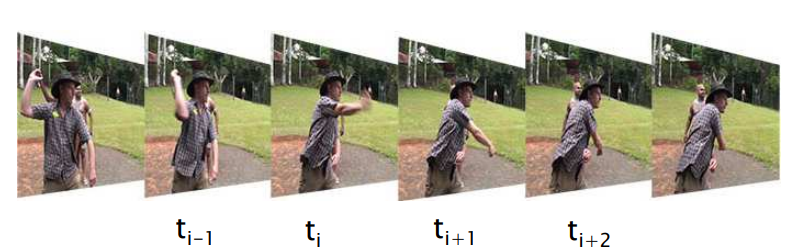
\includegraphics[scale=0.6]{img/video.png}
\end{figure}

\noindent
A video is a 3D signal: $(x,y)$ are the \textit{spatial coordinate} while $t$ is the \textit{temporal coordinate}, fixing the variable $t$ you obtain an image. It is remarkable that new technologies are needed to treat them! An important aspect to be formalized in HAR is the \textbf{time interval} across which the action happens. This can be short (for example an athlete doing squats) or long (a particular action in a football match). \\
We can say that \textbf{Action Recognition} is a computer vision task whose input is a video while the output is the \textit{action label}. Moreover, there different \textit{level of semantics}: action (walking), activity(talking on the phone), event (a birthday part, a soccer game)... where each can be included in the one of an upper semantica level.

We have understood that recognizing human actions is not a trivial task, but \textbf{what is the motivation for doing this?} There are several fields in which such a computer vision task plays an important role: in \textit{robotics} for human-robot interaction and for robot learning, in \textit{smart video-survelillance system} for detecting burglary (anomaly detection), for tagging/summarizing videos an so on. Recognizing actions is useful also for \textit{home monitoring}. \\
We have said that classifying a video is \textbf{challenging}. The following are the main motivations.

\subsection{Challenges in Action Recognition}
\begin{enumerate}
    \itemsep-0.2em
    \item People of which track the acrivity can appear \textbf{at different scales} in different videos; 
    \item In a video scene there could be \textbf{occlusion} in the sense that actions may not be fully visible due to the presence of obstacles in the environment; 
    \item \textbf{Camera movements} are non-negligible in a context where the whole video is analyzed, this can be hand-held (or worn by the subject) or mounted on something which is moving causing the background of the people moving.
    \item It is not said that the video is \textbf{trimmed} to contain only an action and there is no indication of where in the timeline the action occurs.
\end{enumerate}

\subsection{Datasets for action recognition}
Obtaining training datasets for action recognition is extremely challenging, however there are some datasets which provide a quite solid reference point for addressing such taks. The following is a (non-exhaustive) list of well-known datasets: 
\begin{itemize}
    \itemsep-0.2em
    \item \textsc{HDMB51} (Human Motion DB) it is made up 7K clips from 51 action categories (each with 101 samples), they are taken from public repositories like YouTube; 
    \item \textsc{UCF-101} is another commonly used dataset. It has 13k videos from 101 action categories. There are a lot variations of camera  moriton, object scale and appearance... 
    \item \textsc{Sports 1M} It has 1M sports video from youtube with 487 sports label; 
    \item \textsc{ActivityNet} a dataset of 8 hundred hours of video for human activity understanding; 
    \item \textsc{Kinetics-700} it has 700 classes of human-human or human-object \textit{interactions}.
\end{itemize} 

\section{Approaches to action recognition}

\subsection{Hand-crafted approaches}

\subsubsection{Motion History Images (MHI)}

\subsubsection{Optical flow}

\subsubsection{Dense trajectories}

\subsubsection{Improved dense trajectories}

\subsection{Learning-based approaches}